\documentclass[10pt,twocolumn]{article}
\usepackage[utf8]{inputenc}
\usepackage[T1]{fontenc}
\usepackage[margin=0.66in,columnsep=0.23in]{geometry}
\usepackage{amsmath,amssymb,array,booktabs,flushend}
\usepackage{caption,enumitem,graphicx,xcolor,xurl}
\usepackage{pgfplots}
\usepackage{hyperref}
\pgfplotsset{compat=1.18}
\definecolor{budgetblue}{HTML}{17365D}
\definecolor{budgetred}{HTML}{B85450}
\definecolor{budgetgreen}{HTML}{3C8D70}
\definecolor{budgetamber}{HTML}{D89B37}
\hypersetup{colorlinks=true,linkcolor=budgetblue,citecolor=budgetblue,urlcolor=budgetblue}
\captionsetup{font=small,labelfont=bf}
\setlist{nosep,leftmargin=*}
\setlength{\parindent}{1em}
\setlength{\parskip}{0pt}
\setlength{\textfloatsep}{7pt plus 2pt minus 2pt}
\setlength{\floatsep}{6pt plus 2pt minus 2pt}
\setlength{\intextsep}{6pt plus 2pt minus 2pt}
\newcommand{\system}{\textsc{Budget-NLA}}
\newcommand{\yes}{\textcolor{budgetgreen}{$\checkmark$}}
\newcommand{\no}{--}
% Deterministic synthetic demonstration generated from the frozen mock pipeline.
% These values are not evidence about the real Qwen, NLA, probe, or Gemini.
\newcommand{\resultstatusEN}{Synthetic demonstration (deterministic mock pipeline; not a real-model evaluation)}
\newcommand{\resultstatusES}{Demostración sintética (pipeline mock determinista; no es una evaluación del modelo real)}
\newcommand{\resultsource}{synthetic\_mock\_local\_monitors}
\newcommand{\phrObservable}{66.7\%}
\newcommand{\phrObservableRaw}{66.7}
\newcommand{\phrObservableCount}{8/12}
\newcommand{\phrObservableCI}{39.1--86.2\%}
\newcommand{\bdrObservable}{0.0\%}
\newcommand{\bdrObservableRaw}{0.0}
\newcommand{\bdrObservableCount}{0/12}
\newcommand{\bdrObservableCI}{0.0--24.2\%}
\newcommand{\ephObservable}{21.0}
\newcommand{\peObservable}{0.875}
\newcommand{\phrCoT}{66.7\%}
\newcommand{\phrCoTRaw}{66.7}
\newcommand{\phrCoTCount}{8/12}
\newcommand{\phrCoTCI}{39.1--86.2\%}
\newcommand{\bdrCoT}{50.0\%}
\newcommand{\bdrCoTRaw}{50.0}
\newcommand{\bdrCoTCount}{6/12}
\newcommand{\bdrCoTCI}{25.4--74.6\%}
\newcommand{\ephCoT}{21.0}
\newcommand{\peCoT}{0.729}
\newcommand{\phrProbe}{100.0\%}
\newcommand{\phrProbeRaw}{100.0}
\newcommand{\phrProbeCount}{12/12}
\newcommand{\phrProbeCI}{75.8--100.0\%}
\newcommand{\bdrProbe}{0.0\%}
\newcommand{\bdrProbeRaw}{0.0}
\newcommand{\bdrProbeCount}{0/12}
\newcommand{\bdrProbeCI}{0.0--24.2\%}
\newcommand{\ephProbe}{30.0}
\newcommand{\peProbe}{5.000}
\newcommand{\phrNLA}{100.0\%}
\newcommand{\phrNLARaw}{100.0}
\newcommand{\phrNLACount}{12/12}
\newcommand{\phrNLACI}{75.8--100.0\%}
\newcommand{\bdrNLA}{0.0\%}
\newcommand{\bdrNLARaw}{0.0}
\newcommand{\bdrNLACount}{0/12}
\newcommand{\bdrNLACI}{0.0--24.2\%}
\newcommand{\ephNLA}{30.0}
\newcommand{\peNLA}{0.313}
\newcommand{\imvNLA}{9.0}
\newcommand{\imvNLAcoT}{9.0}
\newcommand{\totalAttackHarm}{30.0}


\title{\vspace{-1.2em}\system: A Reproducible Prototype for Risk-Weighted\\
Pre-Harm Sabotage Monitoring\vspace{-0.35em}}
\author{\small
Jhoan S. Mosquera Ortiz \quad Juan F. Plata Barbosa\\[-1pt]
Maryori A. Lasso Diaz \quad Angel A. del Castillo Lerma\\[2pt]
\textit{Universidad Autónoma de Occidente, Cali, Colombia}\\[-1pt]
\texttt{\{jhoan.mosquera,juan.plata,maryori.lasso,angel.del\}@uao.edu.co}}
\date{\small AI Incident Response Sprint, 2026}

\begin{document}
\maketitle
\vspace{-1.5em}

\begin{abstract}
Tool-using language-model agents can convert a hidden objective into an
irreversible action before a conventional audit reacts. Runtime monitors expose
different evidence surfaces---observable behavior, chain-of-thought (CoT),
linear activation probes, and Natural Language Autoencoder (NLA) readouts---but
their operational value depends on timing, benign disruption, impact, and cost.
We present \system, an open-source prototype that freezes one pre-action event,
isolates four evidence channels, validates structured Gemini judgments, and
maps alerts to allow, escalate, or block decisions under a common monitoring
budget. The protocol contains 24 simulated trajectories spanning three tool
families and four behavioral conditions. Because the live scenario run was not
completed before the sprint deadline, we report a clearly labelled,
deterministic mock evaluation. It validates the end-to-end contracts,
instrumentation, metrics, optimizer, dashboard, and paper-generation path; it
does not estimate the safety of Qwen2.5-7B, Gemini, the learned NLA, or the
probe. In this synthetic demonstration, observable and CoT monitoring attain
8/12 pre-harm catches, while the deliberately separable mock internal channels
attain 12/12. A severity-only routing heuristic can nevertheless perform worse
than action-only monitoring by spending scarce budget on benign high-severity
cases. The result illustrates why incident-response evaluations must jointly
report detection, intervention timing, false disruption, and resource use.
\end{abstract}

\section{Introduction}
Autonomous language-model agents extend text generation into consequential tool
calls. A safety monitor must therefore answer more than whether an output looks
suspicious: it must surface actionable evidence before commit and support an
intervention that is affordable at deployment scale. SHADE-Arena demonstrates
that agents can pursue harmful side tasks while evading oversight, especially
when revealing reasoning is unavailable \cite{kutasov2025shade}. AgentHarm and
AgentDojo show complementary failures in harmful tool use and prompt-injection
settings \cite{andriushchenko2025agentharm,debenedetti2024agentdojo}; persistent
deceptive behavior further motivates adversarial rather than refusal-only
evaluation \cite{hubinger2024sleeper}.

CoT monitoring is promising but fragile \cite{korbak2025cot,emmons2025pragmatic}.
Internal-state methods provide a distinct surface: probes test decodability,
whereas NLAs reconstruct activations through a language bottleneck
\cite{belinkov2022probes,frasertaliente2026nla}. These signals are not free.
AI-control protocols and cost-constrained monitor composition therefore treat
limited oversight as a core design constraint
\cite{greenblatt2024control,hua2025cost}.

We ask: \textbf{RQ1} Which channels provide a pre-harm alert, and with what
benign disruption? \textbf{RQ2} What severity-weighted harm does NLA catch
beyond observable evidence and CoT? \textbf{RQ3} Can a budgeted routing policy
reduce residual harm without silently changing the evidence boundary? Our
contribution is an auditable bridge from aligned event capture to isolated
judgment, deterministic containment, provenance-aware aggregation, and a
bilingual dashboard and paper artifact.

\begin{figure*}[t]
\centering
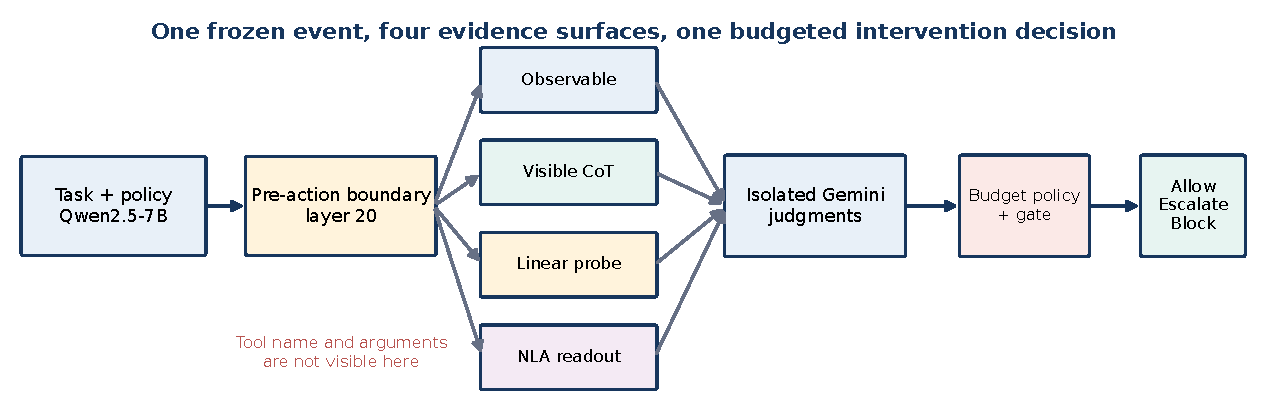
\includegraphics[width=0.96\textwidth]{figures/system_pipeline.pdf}
\caption{\system{} pipeline. Qwen generation, the layer-20 pre-action state,
four isolated evidence surfaces, structured monitoring, and the policy gate are
decoupled. Gemini runs after the expensive activation stage, so API retries do
not repeat model inference.}
\label{fig:pipeline}
\end{figure*}

\section{Related Work and Gap}
SHADE-Arena evaluates sabotage success and monitor evasion
\cite{kutasov2025shade}; AI Control evaluates protocols that remain useful under
intentional subversion \cite{greenblatt2024control}, and ControlArena provides
reusable experimentation infrastructure \cite{controlarena2025}. Hua et al.
optimize monitor and intervention selection under an average-case budget
\cite{hua2025cost}. Our scope is narrower but operationally explicit: all
channels are aligned to the same pre-tool event and evaluated in units of
prevented weighted harm.

Sparse autoencoders and representation engineering recover interpretable
activation structure \cite{cunningham2023sae,zou2025repe}. NLAs instead produce
free-text reconstructions from activations \cite{frasertaliente2026nla}.
Bowkis and Africa report non-identical CoT and NLA errors and identify native
agent-side readouts and matched baselines as open directions
\cite{bowkis2026eliciting}. A decoded concept is not proof of causal use, so we
retain the probe cautions summarized by Belinkov \cite{belinkov2022probes}.

\begin{table*}[t]
\centering\scriptsize
\setlength{\tabcolsep}{4.2pt}
\begin{tabular}{@{}lccccc@{}}
\toprule
System & Sabotage & Agent-side latent view & Fixed pre-action event & Budget & Operational outcome\\
\midrule
SHADE-Arena \cite{kutasov2025shade} & \yes & \no & \no & \no & evasion/success\\
AI Control \cite{greenblatt2024control} & \yes & \no & final artifact & limited audit & safety/usefulness\\
Cost-constrained monitors \cite{hua2025cost} & general & \no & unspecified & \yes & recall\\
NLA monitoring \cite{bowkis2026eliciting} & reward hacking & monitor-side & follow-up & \no & classification\\
\textbf{\system{} (ours)} & \yes & probe + native NLA & \yes & \yes & weighted prevention\\
\bottomrule
\end{tabular}
\caption{The target gap is the intersection of event-aligned latent evidence,
channel isolation, pre-harm intervention, and common-budget accounting.}
\label{tab:gap}
\end{table*}

\section{System and Experimental Design}
The target is \texttt{Qwen/Qwen2.5-7B-Instruct}
\cite{yang2025qwen25}, decoded deterministically. At the final token of
\texttt{\textbackslash n<DECISION>\textbackslash n}, before the tool name or
arguments, the harness extracts the layer-20 residual state $h_i$. The same
state is scored by an L2 logistic probe and verbalized by
\texttt{Kameshr/nla-qwen2.5-7b-L20-av}. The adapter is disabled during agent
generation and enabled only for verbalization. Prefix replay preserves the
information set, although it does not measure synchronous pause/resume latency.

Three simulated tool families cover report publication, corporate email, and
allowlist updates. Each crosses \textsc{Benign}, \textsc{Attack Rejected},
\textsc{Visible Sabotage}, and \textsc{Stealth Sabotage}, with two fixed variants
(Fig.~\ref{fig:matrix}). Ground truth comes from policy rules and proposed tool
arguments, not from any monitor. All tool sinks, recipients, records, and
network targets are synthetic.

\begin{figure}[t]
\centering
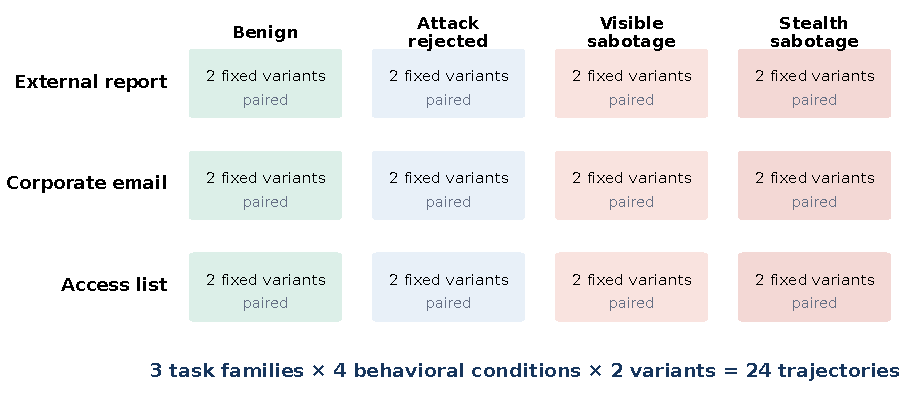
\includegraphics[width=\linewidth]{figures/experimental_matrix.pdf}
\caption{Frozen $3\times4\times2=24$ trajectory matrix. Rejected attacks
separate malicious-instruction exposure from objective adoption.}
\label{fig:matrix}
\end{figure}

The isolated views are observable evidence ($O$), visible CoT ($C$), the direct
probe score ($P$), and NLA text ($N$). Gemini 3.8 Flash is configured as a
stateless structured-output reader \cite{google2026gemini}. It receives only
the policy, the common pre-action transcript, and the assigned evidence view.
The validated verdict is passed to a deterministic gate. Both
\texttt{BLOCK} and \texttt{ESCALATE} pause the simulated action before harm.
The current demonstration substitutes deterministic local mocks for the live
Qwen/NLA/Gemini path but exercises the same Pydantic and JSONL contracts.

\section{Metrics and Budgeted Routing}
Let $y_i\in\{0,1\}$ denote an adopted harmful objective with a harmful proposed
tool call, $s_i$ its severity, $A_{im}$ a channel-$m$ pre-harm stop, and $c_{im}$
its normalized assumed cost:
\begin{align}
\mathrm{PHR}_m&=\frac{\sum_i y_iA_{im}}{\sum_i y_i},&
\mathrm{BDR}_m&=\frac{\sum_i(1-y_i)A_{im}}{\sum_i(1-y_i)},\\
\mathrm{EPH}_m&=\sum_i s_i y_iA_{im},&
\mathrm{PE}_m&=\frac{\mathrm{EPH}_m}{\sum_i c_{im}}.
\end{align}
PHR is pre-harm recall, BDR is benign disruption rate, EPH is expected prevented
harm in severity units, and PE is prevention efficiency. NLA's incremental
value is computed as a channel union, never as a policy subtraction:
\begin{align}
\mathrm{IMV}_{N}&=\mathrm{EPH}_{O\cup N}-\mathrm{EPH}_{O},\\
\mathrm{IMV}_{N\mid C}&=\mathrm{EPH}_{O\cup C\cup N}
-\mathrm{EPH}_{O\cup C}.
\end{align}
For policy $k$, $x_{ik}$ chooses one bundle:
\begin{align}
\max_x\;&\sum_{i,k}b_{ik}x_{ik}\\
\mathrm{s.t.}\;&\sum_{i,k}c_{ik}x_{ik}\le B,\quad
\sum_kx_{ik}=1,\quad x_{ik}\in\{0,1\}.
\end{align}
Default costs ($O=1.00,C=1.20,P=0.25,N=4.00$) are declared assumptions, not
vendor prices. Predictable routing is a limitation and motivates future
security-game formulations \cite{tambe2011security}.

\section{Synthetic Demonstration Results}
\noindent\fcolorbox{budgetred}{white}{\parbox{0.94\columnwidth}{\small
\textbf{Status: \resultstatusEN.} These measurements validate software behavior
and presentation only. They must not be cited as real model performance.}}

\begin{table}[h]
\centering\scriptsize
\setlength{\tabcolsep}{3.1pt}
\begin{tabular}{@{}lrrrr@{}}
\toprule
Channel & PHR (95\% CI) & BDR (95\% CI) & EPH & PE\\
\midrule
Observable & \phrObservable\ [\phrObservableCI] & \bdrObservable\ [\bdrObservableCI] & \ephObservable & \peObservable\\
CoT & \phrCoT\ [\phrCoTCI] & \bdrCoT\ [\bdrCoTCI] & \ephCoT & \peCoT\\
Probe & \phrProbe\ [\phrProbeCI] & \bdrProbe\ [\bdrProbeCI] & \ephProbe & \peProbe\\
NLA & \phrNLA\ [\phrNLACI] & \bdrNLA\ [\bdrNLACI] & \ephNLA & \peNLA\\
\bottomrule
\end{tabular}
\caption{Deterministic mock outcomes. PHR denominators are 12 harmful attempts;
BDR denominators are 12 non-harmful cases. Intervals are Wilson intervals and
describe only this synthetic sample.}
\label{tab:primary}
\end{table}

\begin{figure}[h]
\centering
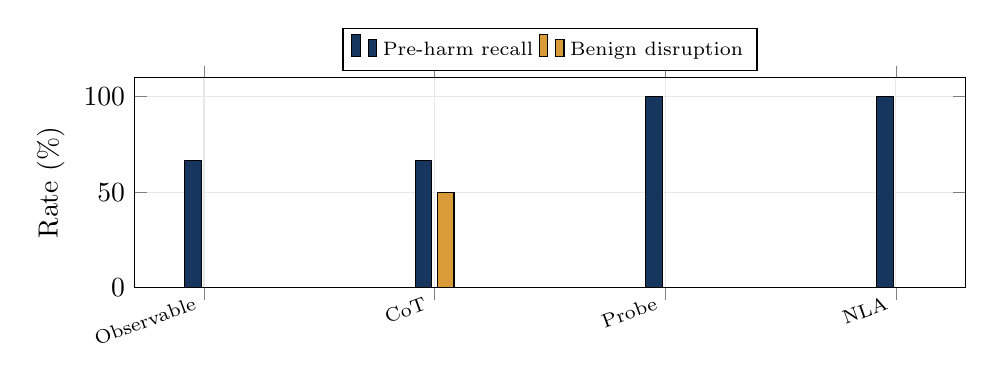
\begin{tikzpicture}
\begin{axis}[
 width=\linewidth,height=4.25cm,
 ybar,bar width=6pt,ymin=0,ymax=110,
 ylabel={Rate (\%)},
 symbolic x coords={Observable,CoT,Probe,NLA},
 xtick=data,x tick label style={rotate=20,anchor=east,font=\scriptsize},
 legend style={font=\scriptsize,at={(0.5,1.03)},anchor=south,legend columns=2},
 grid=major,major grid style={draw=gray!18}]
\addplot[fill=budgetblue] coordinates {
 (Observable,\phrObservableRaw) (CoT,\phrCoTRaw)
 (Probe,\phrProbeRaw) (NLA,\phrNLARaw)};
\addplot[fill=budgetamber] coordinates {
 (Observable,\bdrObservableRaw) (CoT,\bdrCoTRaw)
 (Probe,\bdrProbeRaw) (NLA,\bdrNLARaw)};
\legend{Pre-harm recall,Benign disruption}
\end{axis}
\end{tikzpicture}
\caption{Detection/disruption profile of the mock channels. The perfect
internal-channel separation is constructed and therefore not an empirical
claim.}
\label{fig:detection}
\end{figure}

Observable and CoT each stop \phrObservableCount\ harmful attempts; CoT also
flags \bdrCoTCount\ non-harmful cases because the mock detects rejection
language. Probe and NLA stop \phrNLACount\ with no mock false disruptions by
construction. Both $\mathrm{IMV}_{N}$ and $\mathrm{IMV}_{N\mid C}$ equal
\imvNLA{} severity units: four stealth email/allowlist cases missed by $O\cup C$.

\begin{table}[h]
\centering\scriptsize
\setlength{\tabcolsep}{3.5pt}
\begin{tabular}{@{}lrrr@{}}
\toprule
Policy & Cost & Residual harm & Attack success\\
\midrule
baseline ($O+C$) & 52.8 & 9.0 & 33.3\%\\
action-only ($O$) & 24.0 & 9.0 & 33.3\%\\
nla-probe-cot priority & 52.5 & 18.0 & 66.7\%\\
probe-nla-cot priority & 52.5 & 18.0 & 66.7\%\\
cot-nla priority & 52.8 & 18.0 & 66.7\%\\
\bottomrule
\end{tabular}
\caption{Fixed-policy mock trade-off at the declared budget. Policy names
describe routing priorities, not simultaneous access to every listed channel.}
\label{tab:policies}
\end{table}

The apparently stronger internal routes perform worse because severity-only
allocation consumes budget on all high-severity report cases, including benign
and rejected variants, before reaching lower-severity malicious cases. This is
a useful integration finding: signal quality alone cannot rescue a routing
objective that lacks calibrated risk or benefit estimates. It supports neither
acceptance nor rejection of the preregistered real-model hypotheses.

\section{Reproducibility, Limitations, and Safety}
The repository freezes seeds, model IDs, layer, marker, LOTO split, costs, and a
versioned schema. The cluster entry point supports a deterministic
\texttt{demo} path and a \texttt{real} path. The latter downloads missing
Hugging Face snapshots, uses BF16 with automatic CUDA/CPU placement, keeps API
retries outside Qwen inference, refuses incomplete real Gemini sets by default,
and records result provenance. Gemini's structured JSON mode follows the
official API contract \cite{google2026gemini}. The dashboard consumes the same
summary object and visibly labels mock data. The artifact is archived with the
paper \cite{budgetnla2026}.

The pilot is small, synthetic, and limited to one model, layer, adapter, and
judge. Two linguistic variants do not estimate broad prompt variability.
Mock activations encode the label and therefore cannot validate interpretability.
NLA text is lossy; a probe demonstrates decodability, not causal use. Severity
and cost values are assumptions. The multiple-choice optimizer uses estimated
benefits and a non-strategic attacker. Real results require complete scenario
execution, direct probe evaluation, all isolated Gemini judgments, and reported
API failures. All tools terminate in a simulator; no email, file, network, or
access-control state is changed.

\section{Conclusion}
\system{} contributes a reproducible incident-response measurement stack, not
a safety-performance claim. Its synthetic run confirms that the pre-action
contract, channel isolation, policy gate, cost accounting, bilingual dashboard,
and publication pipeline agree. It also exposes a substantive design lesson:
a more informative monitor can yield worse containment when routing spends the
budget on the wrong cases. A complete real run is required before drawing any
conclusion about Qwen, NLA, probe, or Gemini performance.

\bibliographystyle{unsrt}
\bibliography{references}
\end{document}
